\documentclass{beamer}

\usepackage{lmodern}
\usepackage[spanish]{babel}
\usepackage[utf8]{inputenc}
\usepackage[T1]{fontenc}
\usepackage{hyperref}
\usepackage{bm}

\newcommand{\hrefCustom}[2]{\href{#1}{\color{blue} #2}}

\setlength{\parskip}{1em}
\usetheme{Warsaw}

\title{Vulnerabilidades usando SDR}
\subtitle{SDR = Software Defined Radio}
\author{Carlos Ledesma Peña}
\institute{Trabajo de Fin de Grado, E.T.S. de Ingeniería Informática}
\date{}

%\AtBeginSection[]
%{
%	\begin{frame}[shrink=37]
%		\frametitle{Índice}
%		\vspace{2em}
%		\tableofcontents[currentsection]
%	\end{frame}
%}

\AtBeginSubsection[]
{
	\begin{frame}[shrink=37]
		\frametitle{Índice}
		\vspace{2em}
		\tableofcontents[currentsection,currentsubsection]
	\end{frame}
}

% To include images from 'images' directory
\graphicspath{ {./images/} }

\begin{document}

\begin{frame}
\titlepage
\end{frame}

\section{Introducción}

\subsection{Justificación}

\begin{frame}{¿Por qué es importante la seguridad informática?}

La mayoría de los sistemas informáticos en producción no se encuentran aislados, sino que automatizan la gestión de la información en otros sistemas, información sensible...
\begin{itemize}
	\item \textbf{Correos electrónicos:} ¿Y si terceros pudiesen leer nuestra correspondencia electrónica? (confidencialidad).
	\item \textbf{Transferencias bancarias:} ¿Y si se pudiese cambiar el destinatario de una transferencia bancaria? (integridad).
	\item \textbf{Gestión de intervenciones de ambulancias:} ¿No morirían personas si las ambulancias llegan tarde por estar el sistema caído? (disponibilidad).
\end{itemize}

\end{frame}

\begin{frame}{La preocupación por la radiocomunicación}

\begin{columns}

\begin{column}{.25\textwidth}
\begin{center}

\includegraphics[scale=0.1]{Question-Mark.jpg}
\end{center}
\end{column}

\begin{column}{.66\textwidth}
\bigskip
\textbf{¿Debe preocuparnos la seguridad de los sistemas que usan radiocomunicación?}
\end{column}

\end{columns}

\end{frame}

\begin{frame}{Características de un ataque}

Un ataque puede ser llevado a distancia y anonimamente (y a más distancia de lo normal para ese sistema).

\bigskip

\begin{columns}

\begin{column}{.66\textwidth}
\begin{center}
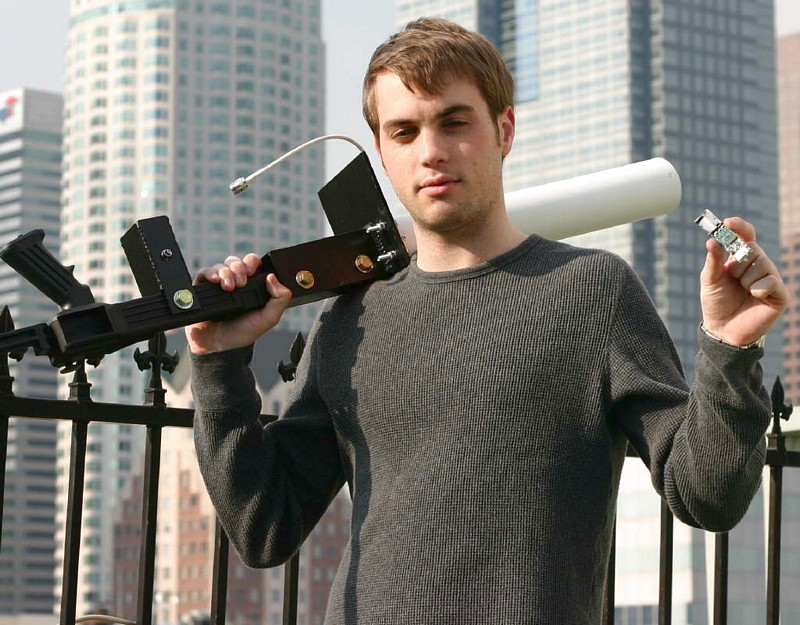
\includegraphics[scale=0.5]{bluetooth_sniper_rifle.jpg}
\end{center}
\end{column}

\begin{column}{.40\textwidth}
\emph{John Hering con su rifle BlueSniper, con el que es posible interactuar con dispositivos Bluetooth a más de kilómetro y medio de distancia.}
\end{column}

\end{columns}

\end{frame}

\begin{frame}{Uso y posible abuso}

El número de dispositivos que usan radiocomunicación aumenta con el tiempo:

\begin{itemize}
	\item Un router \emph{Wi-Fi}, unos auriculares \emph{Bluetooth}, un pasaporte con \emph{RFID}, un teléfono móvil, otros dispositivos usando protocolos propietarios...
\end{itemize}

Las herramientas de ataque cada vez son más baratas y más fáciles de usar:

\begin{itemize}
	\item Dispositivos usando tecnología SDR por apenas 20 dólares, y software gratuito y relativamente simple con interfaz gráfica.
\end{itemize}

\end{frame}

\subsection{¿Qué es SDR?}

\begin{frame}{Vulnerabilidad, radio y sofware defined radio}

Antes de empezar, es conveniente dar algunas definiciones:

\begin{itemize}
	\item \textbf{Vulnerabilidad: } Error de diseño o implementación en un sistema que puede ser aprovechado para comprometer la confidencialidad, integridad o disponibilidad de éste.
	\item \textbf{Radio:} Tecnología que transmite o recibe sin cables radiación electromagnética para transferir información. También se llama así al sistema o dispositivo incorporando esta tecnología.
	\item \textbf{Software defined radio:} Radio en la cual algunas o todas las funciones de las capas físicas están implementadas en software.
\end{itemize}

\end{frame}

\begin{frame}{En la práctica}

La mayoría de los dispositivos SDR de consumo que se utilizan junto con un ordenador personal, básicamente sintonizan a una frecuencia y capturan una banda determinada, digitalizándola y enviándola al PC, donde se hará el resto de operaciones (separación en canales, demodulación, decodificación, división en tramas...).

\begin{center}
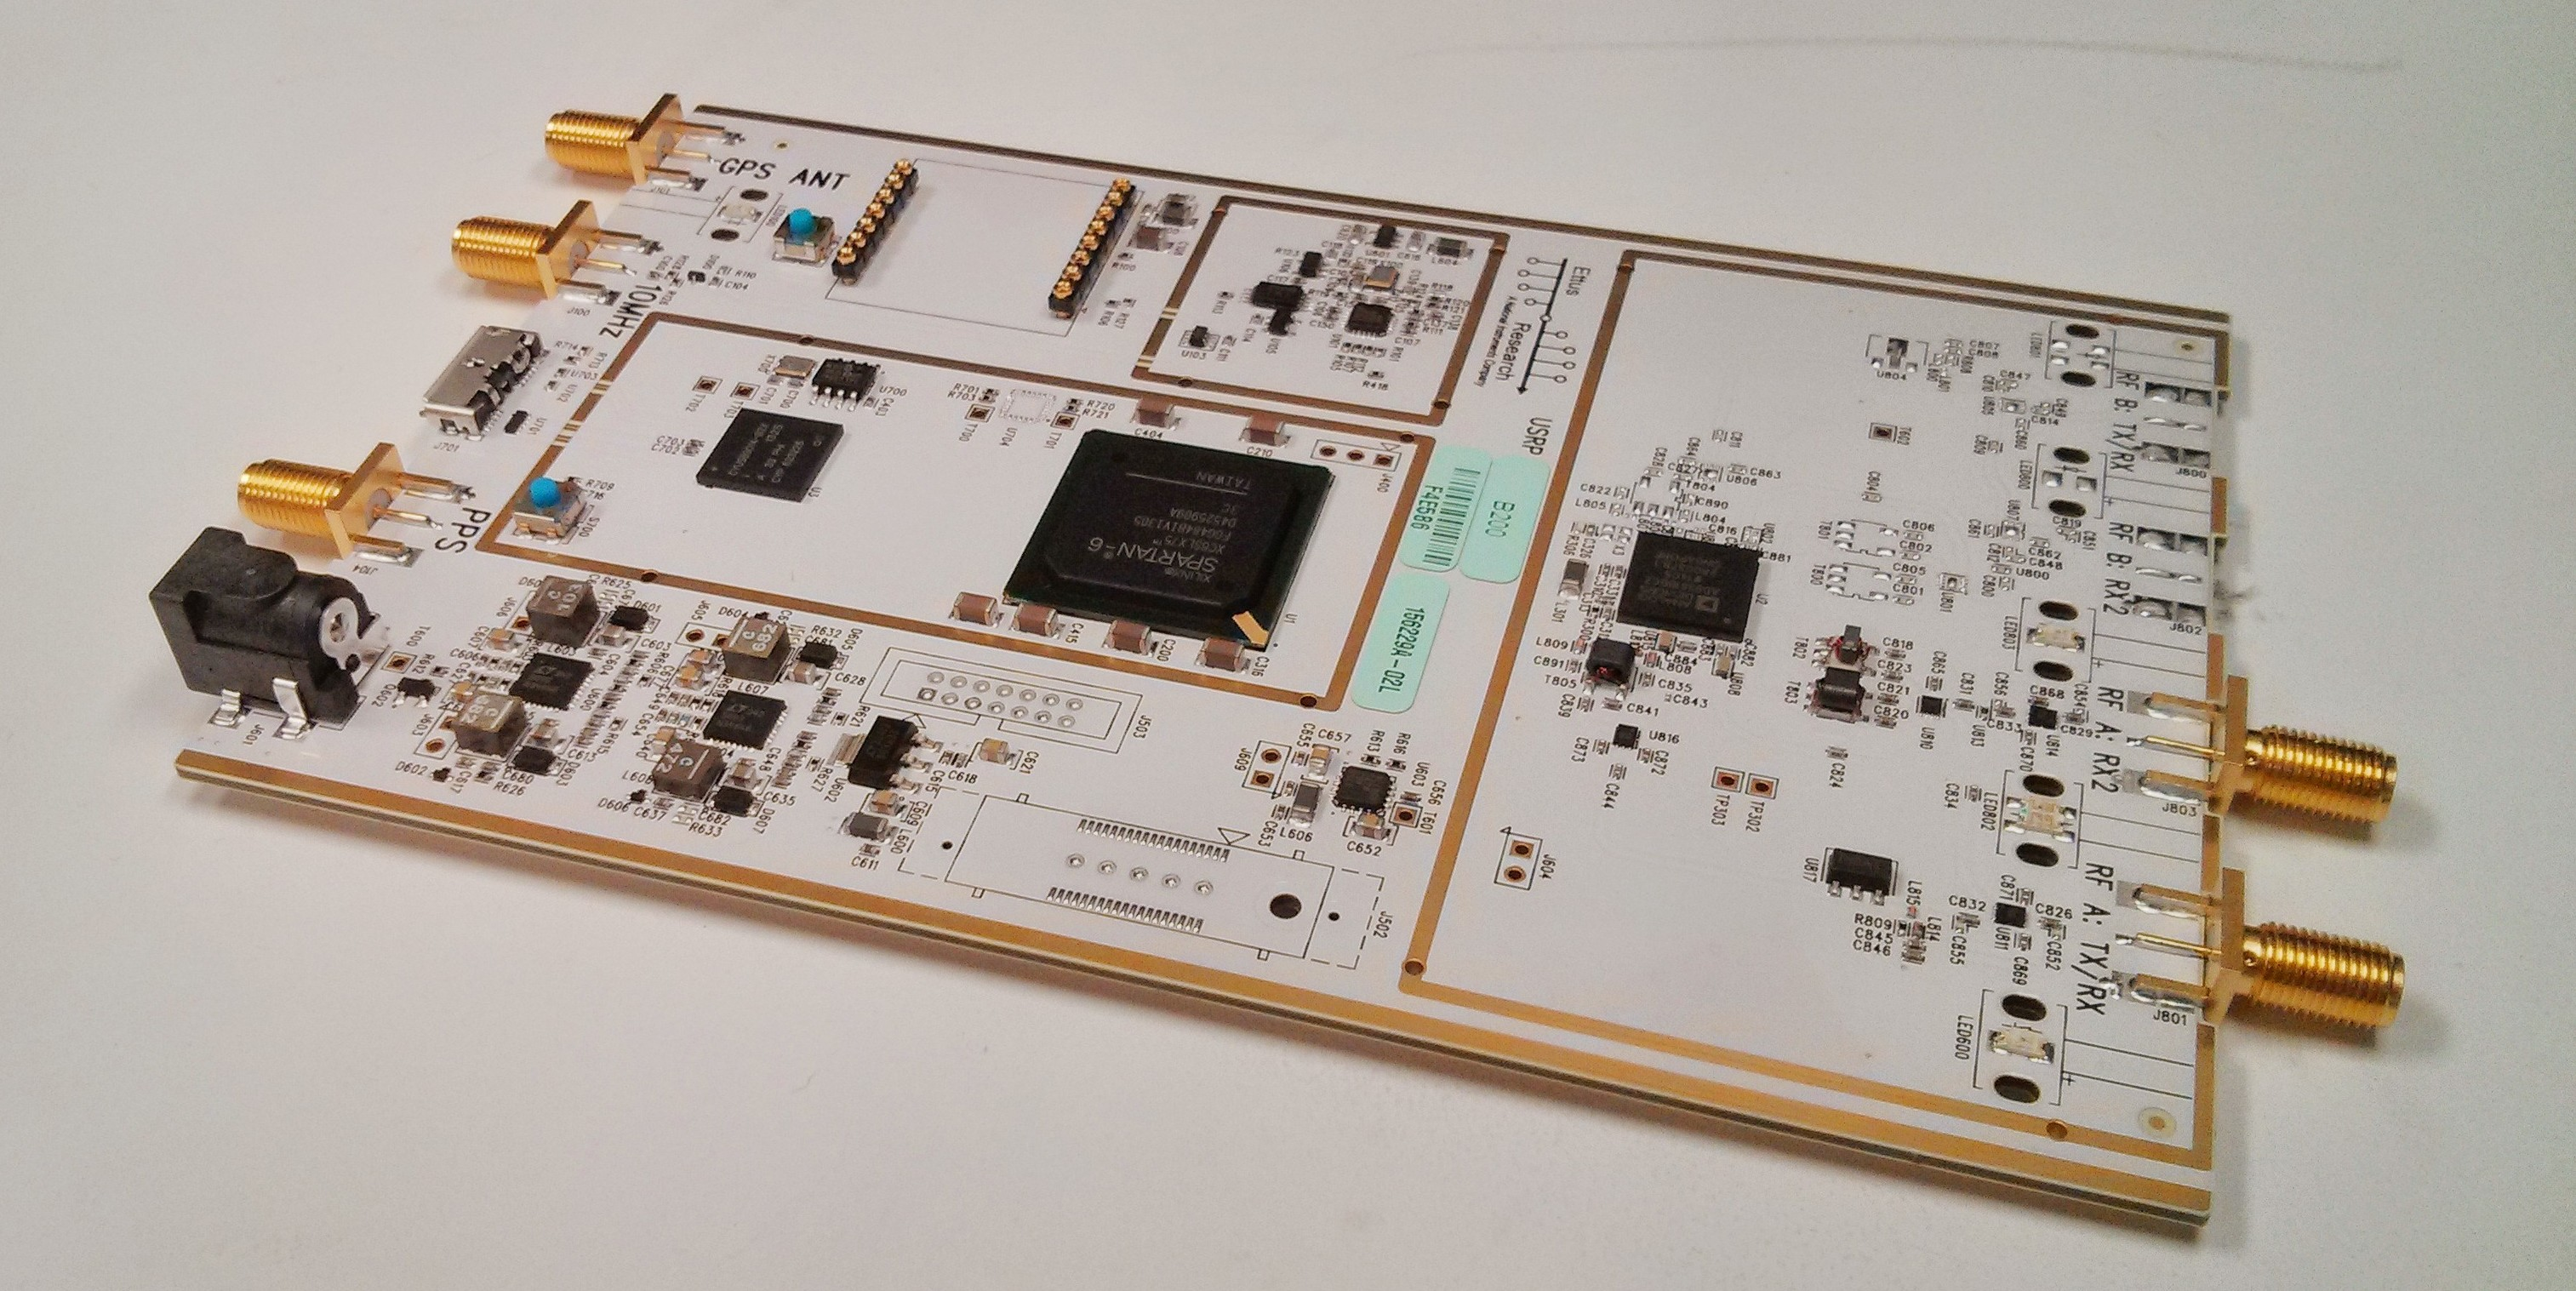
\includegraphics[scale=0.06]{USRP-B200.jpg}
\end{center}

\end{frame}

\section{Evolución en el tiempo de la tecnología SDR}

\begin{frame}{Comienzos}

\begin{itemize}
	\item \textbf{Década de los 70:} Interés por parte del sector de defensa en un sistema de radio flexible.
	\item \textbf{1984:} Prototipo primitivo de SDR, únicamente recepción.
	\item \textbf{1991:} Comienzo del programa \emph{SPEAKeasy}, que buscaba crear un dispositivo único que fuese compatible con varios dispositivos existentes.
	\item \textbf{1998:} Primera versión de \emph{SignalMaster}, una de las primeras plataformas de desarrollo SDR.
	\item \textbf{2001:} Creación de \emph{GNU Radio}, el entorno de desarrollo open source más importante.
	\item \textbf{2006:} Salida al mercado de \emph{Small Form Factor}, la primera plataforma de desarrollo SDR completa y autónoma.
\end{itemize}

\end{frame}

\subsection{Comienzos}

\begin{frame}{Comienzos}

\begin{itemize}
	\item \textbf{Década de los 70:} Interés por parte del sector de defensa en un sistema de radio flexible.
	\item \textbf{1984:} Prototipo primitivo de SDR, únicamente recepción.
	\item \textbf{1991:} Comienzo del programa \emph{SPEAKeasy}, que buscaba crear un dispositivo único que fuese compatible con varios dispositivos existentes.
	\item \textbf{1998:} Primera versión de \emph{SignalMaster}, una de las primeras plataformas de desarrollo SDR.
	\item \textbf{2001:} Creación de \emph{GNU Radio}, el kit de desarrollo open source más importante.
	\item \textbf{2006:} Salida al mercado de \emph{Small Form Factor}, la primera plataforma de desarrollo SDR completa y autónoma.
\end{itemize}

\end{frame}

\subsection{Seguridad}

\begin{frame}{Seguridad}

\begin{itemize}
	\item \textbf{2005:} Versión mejorada de \emph{BlueSniper}.
	\item \textbf{2007:} Ataque sobre teclados inalámbricos.
	\item Ataque sobre el pasaporte europeo.
	\item \textbf{2008:} Michael Ossmann repasa en Black Hat sobre el estado de la seguridad de las radiocomunicaciones, y advierte que SDR accesible es peligroso.
	\item Ataque sobre el sistema de tarjetas del metro de Boston y de pago remoto en peajes.
	\item \textbf{2009:} Ataque práctico sobre \emph{GSM}.
	\item \textbf{2010:} Lectura de \emph{RFID} a larga distancia.
	\item \textbf{2011:} Ataque sobre \emph{GRPS/EDGE} y \emph{UMTS/HSPA}.
\end{itemize}

\end{frame}

\subsection{Estado actual}

\begin{frame}{Estado actual}

\begin{itemize}
	\item En 2010, Eric Fry se da cuenta de algo extraño al realizar ingeniería inversa a un \emph{driver} de un dispositivo \emph{USB} para recepción \emph{FM} y \emph{DAB+}. Lo que viaja del dispositivo al PC no es audio, sino muestras de la señal en una etapa intermedia entre la señal de radiofrecuencia y el audio.
	\item En 2012 nace el proyecto \emph{rtl-sdr}, que proporciona una interfaz para usar estos dispositivos como SDR's (sólo recepción, pero muy asequibles).
	\item Interés en integrar SDR en la comunidad de pentesting, con nuevas herramientas que permiten inyectar paquetes de diversos protocolos al vuelo.
\end{itemize}

\end{frame}

\section{Caso práctico}

\subsection{GNU Radio}

\begin{frame}{¿Qué es GNU Radio?}

\emph{GNU Radio} es un entorno de desarrollo \emph{open source} multiplataforma de procesamiento de señales en general, si bien está especializado en SDR, pero no limitado a ello.

\begin{itemize}
	\item Ofrece una interfaz gráfica, \emph{GRC}, además de las interfaces para \emph{Python} y \emph{C++}. La de \emph{Python} es una envoltura de la de \emph{C++}, y la gráfica una envoltura de la de \emph{Python}.
	\item La interfaz gráfica sirve para crear diagramas de flujo, con conexiones entre bloques que representan funciones de procesamiento de señales.
	\item Los bloques pueden ser de entrada o salida, para interactuar con el exterior (parte hardware de SDR, tarjeta de audio, disco duro...), o de entrada y salida, implementando funciones en sí.
\end{itemize}

\end{frame}

\begin{frame}{GRC}

\begin{center}
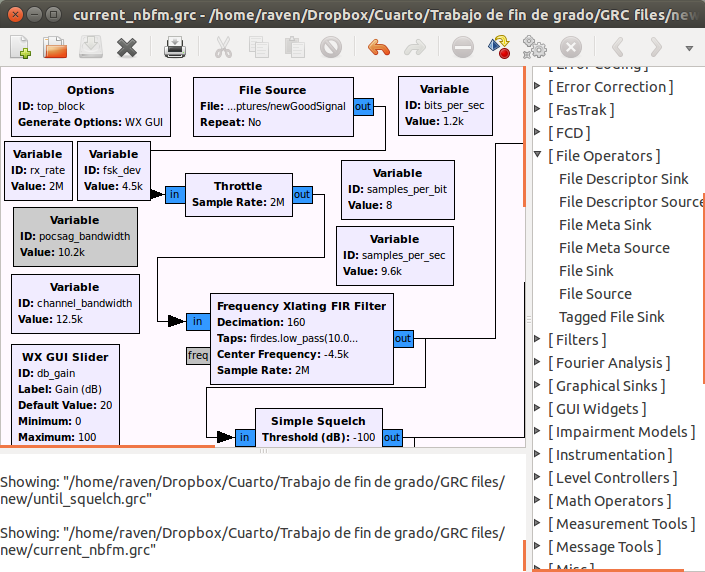
\includegraphics[scale=0.3]{grc.png}
\end{center}

\end{frame}

\subsection{Pager POCSAG}

\begin{frame}{¿Qué es un pager POCSAG?}

\begin{center}
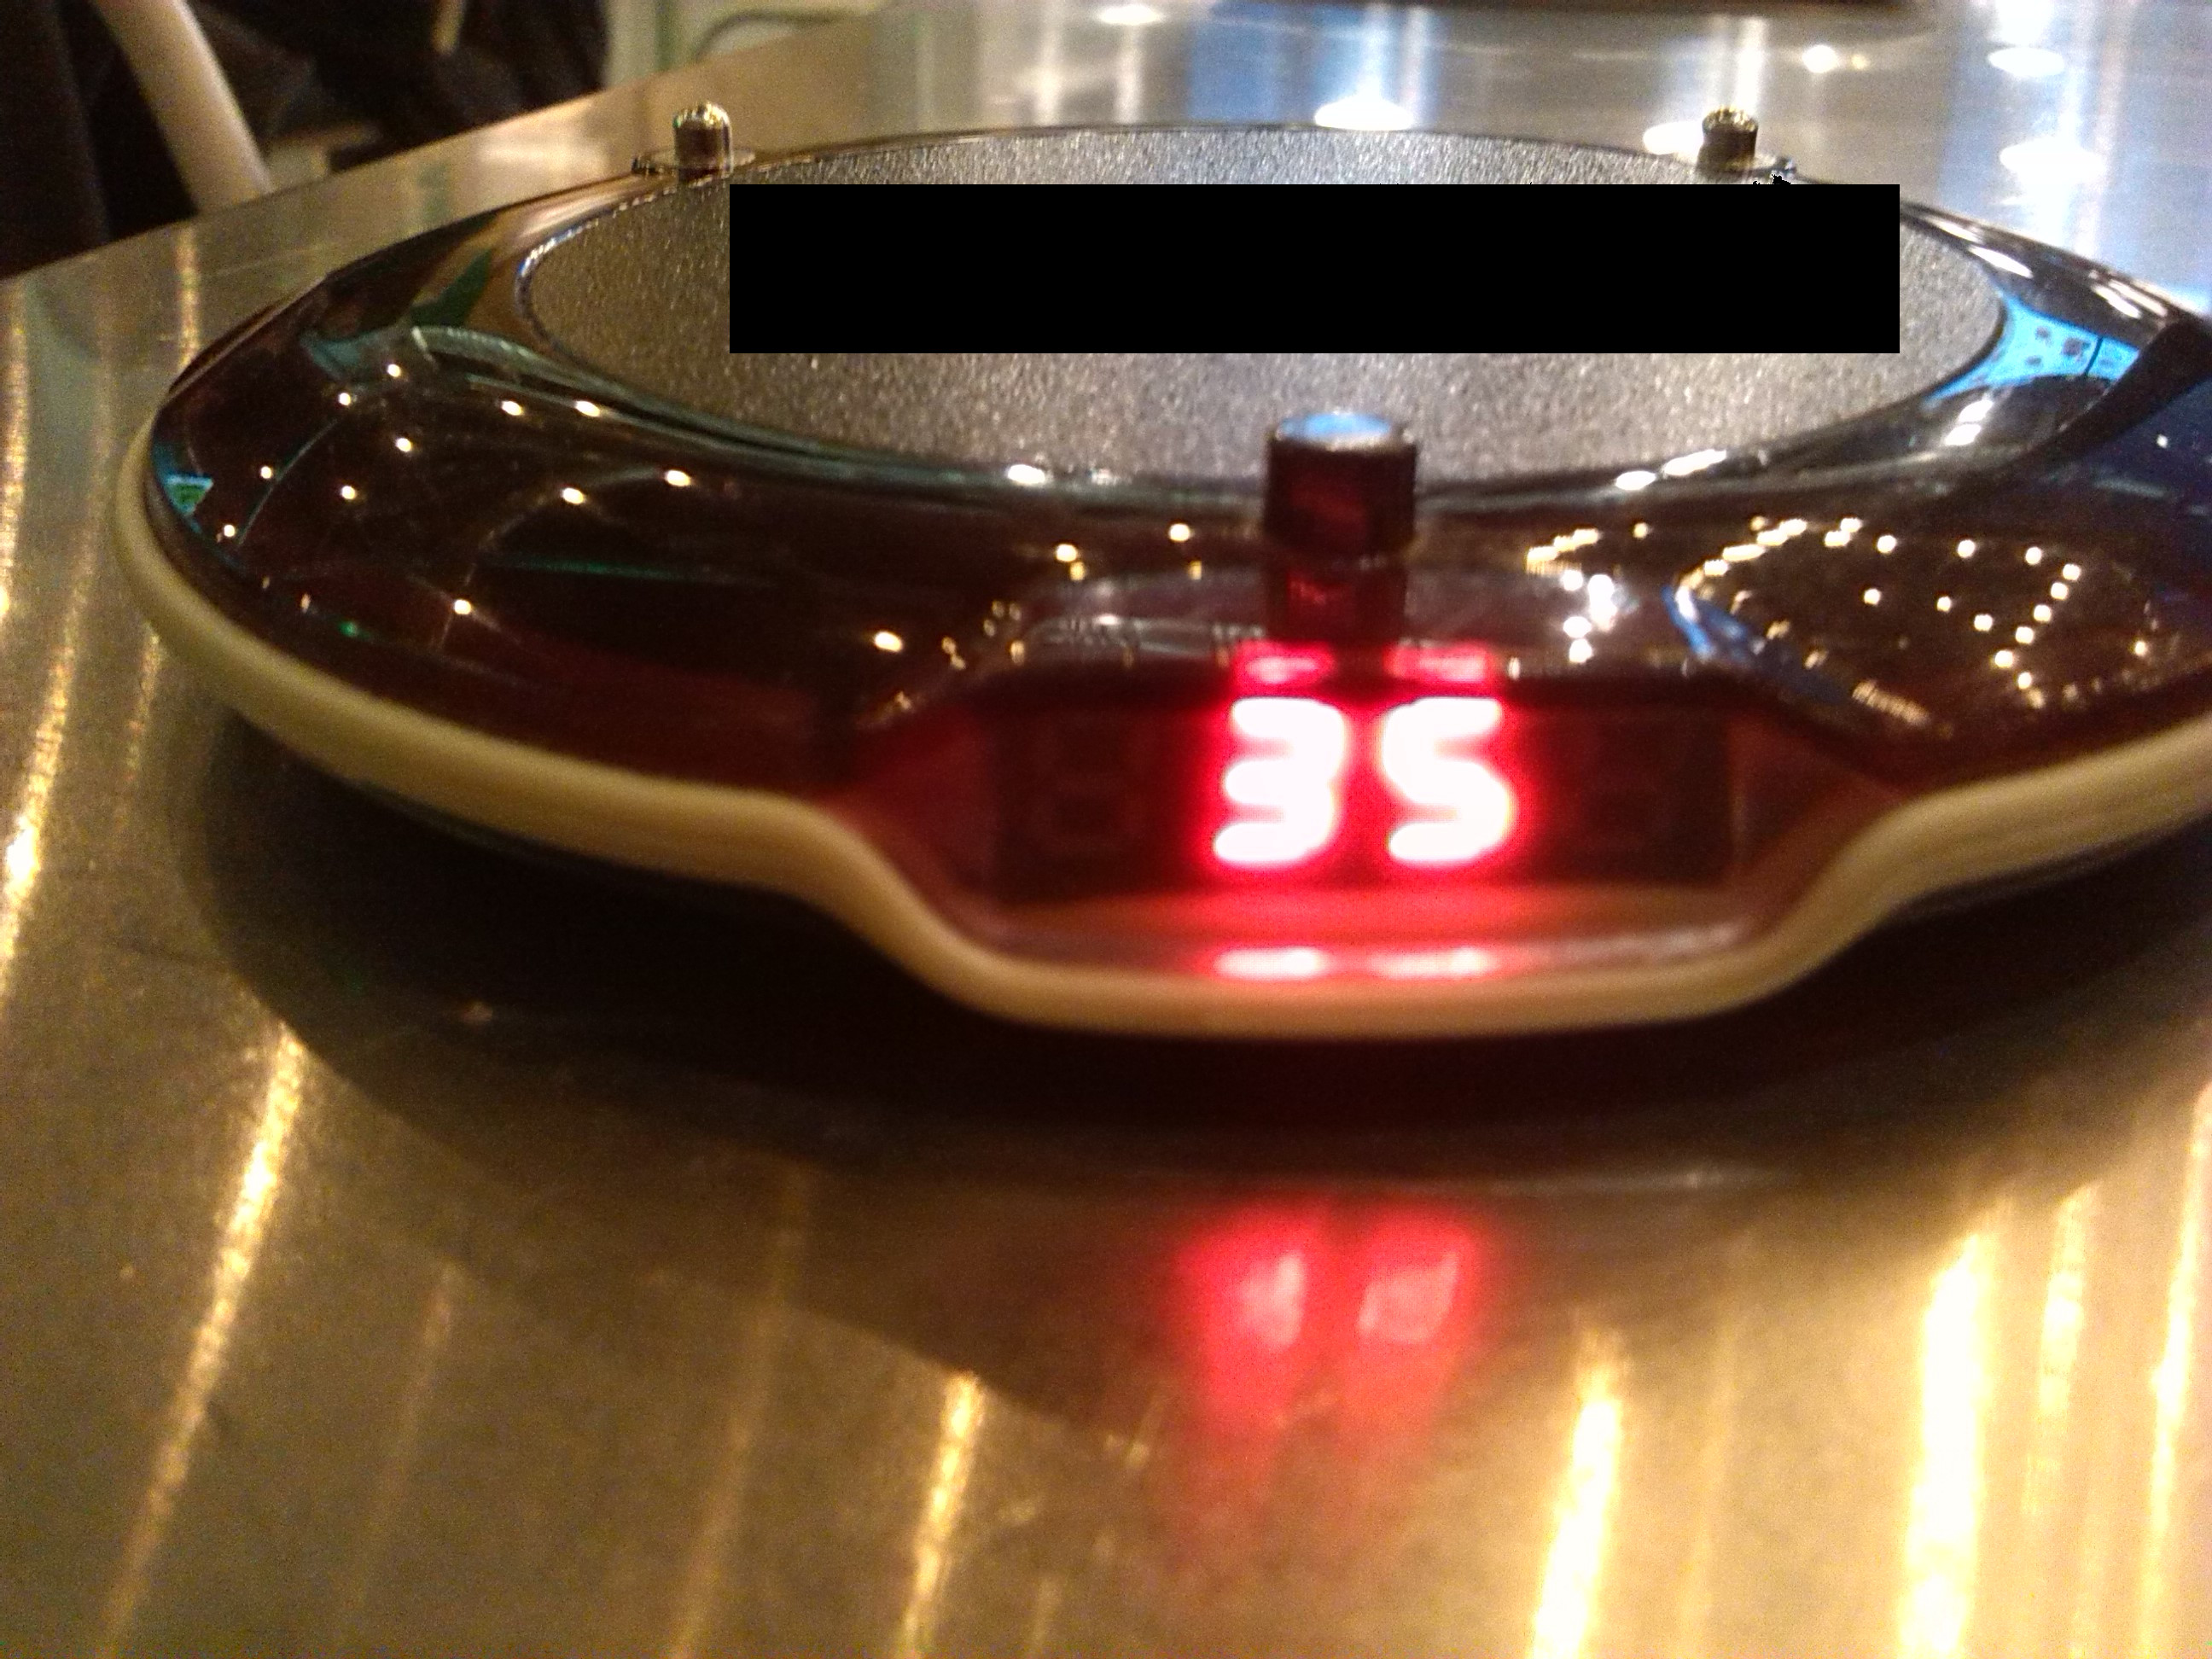
\includegraphics[scale=0.08]{pagerfront.jpg}
\end{center}

\end{frame}

\begin{frame}{Al ataque}

\begin{itemize}
	\item Tras escanear en el rango de frecuencias que menciona el \emph{pager} en su parte de atrás, y los avisos que alcanzo a capturar se emiten en la misma frecuencia.
	\item Construyo el diagrama de flujo (no sin mucho esfuerzo) para decodificar con arreglo al estándar \emph{POCSAG} y efectivamente, se ajusta al estándar. Cada disposivo tiene un ID, y suena cuando se emite el suyo.
	\item Modifico el diagrama de flujo y creo un bloque personalizado para \emph{GRC} para imprimir en consola los ID's según se capturan los avisos.
\end{itemize}

\end{frame}

\begin{frame}{Dificultades encontradas}

\begin{itemize}
	\item Dominio completamente nuevo para mí, y falta de base sólida a la hora de resolver los problemas (días de diagnóstico por problema).
	\item \emph{GRC} no está hecho para aprender a base de prueba y error desde el principio, no es fácil saber qué está fallando ni por qué (curva de aprendizaje elevada).
	\item Limitaciones del hardware, mi portátil usa \emph{USB 2.0}, lo que limita el ancho de banda capturable de una vez, además de no tener potencia de procesamiento suficiente y descartar muestras si se usaban varias operaciones simultáneamente.
\end{itemize}


\end{frame}

\section{Para terminar}

\subsection{Conclusiones}

\begin{frame}{Conclusiones}

\begin{itemize}
	\item Desde el punto de vista económico y humano, es necesario invertir en la seguridad de los sistemas informáticos. No sólo se protege de las malas intenciones, sino de las buenas intenciones equivocadas.
	\item La ''seguridad'' por oscuridad no es seguridad, si un sistema necesita que su forma de funcionar no sea pública para ser seguro, no es seguro igualmente. \emph{Sólo la clave debe ser desconocida para el resto}.
	\item No se le ha prestado suficiente atención a la seguridad de las radiocomunicaciones en el pasado, y ahora se dispone de herramientas basadas en SDR que facilitan aprovecharse de sistemas vulnerables. Hay que prestarle atención desde ya.
\end{itemize}

\end{frame}

\subsection{Utilidades}

\begin{frame}{Utilidades}

\begin{itemize}
\setlength{\itemsep}{12pt}
	\item Aprender conocimientos básicos de radio (inquietud personal).
	\item Incorporar una nueva herramienta de trabajo (es posible que se incorpore en labores de pentesting).
	\item Servir de guía de inicio rápido a SDR a los investigadores del departamento.
	\item Obtener el título de Graduado en Ingeniería Informática.
\end{itemize}

\end{frame}

\begin{frame}

\begin{center}
\textbf{¡Gracias por vuestra atención!}
\end{center}

\end{frame}

\end{document}